\section{Descripción del problema}

\subsection{Análisis en Tiempo Real}

Se planteó la meta de que el algoritmo pueda realizar el seguimiento en tiempo
real, aprovechando que contornos activos, la técnica utilizada para obtener la
posición de los jugadores es lo suficientemente eficiente para funcionar en
tiempo real.

Realizar el seguimiento en tiempo real agrega restricciones fuertes al
problema. Toda técnica tiene un costo de procesamiento, por lo tanto se debe
tener cautela al momento de seleccionar qué procesos de análisis de imagen
pueden ser realizados en los aproximadamente 40 milisegundos que separan un
cuadro de otro al mostrar un video de 24 cuadros por segundo.

\subsection{Supervisión Humana}

% TODO: BULLLLLSHITTTTTT los tanos no tenian 100% automatico?
% Esteban says: No, los tanos tenían fallas en su algoritmo aunque creo
% que era solo con el seguimiento de la pelota. 80% accuracy

% Ahí leí de nuevo y si lo tienen resuelto, sorry.

Respecto a la supervición necesaria, el objetivo que se planteó es igualar y
complementar la información sobre un partido que un operador (o grupo de
operadores) podría obtener de un video.

En el presente trabajo, un supervisor seleccionará inicialmente las posiciones
de los jugadores en la cancha. El algoritmo de contornos activos será
ejecutado para obtener la posición de cada jugador para los cuadros siguientes.
El supervisor corregirá eventuales incorrectas actualizaciones de contornos
activos. Se desea minimizar estas falsas detecciones.

\subsection{Sistema de Cámaras}

Nuestro enfoque consta de un sistema de una única cámara fija, posicionada en
la cancha de tal forma que pueda observar toda la cancha en un solo cuadro. Al
utilizar una única cámara, la resolución adquiere un rol determinante,
dificultando o impidiendo el uso de muchas de las técnicas de seguimiento.

\subsection{Dificultades}

\subsubsection{Corregir la Perspectiva de la Cámara}

La imagen capturada por la cámara es una representación en 2 dimensiones de
la realidad. Nuestro modelo de datos representa cada jugador y la pelota
como un punto en un campo de dos dimensiones, es decir, se descarta el valor
de la altura de cada objeto seguido, ya que no interesa esa información.
Para esto, se aplica una homografía para convertir las coordenadas de un punto de
la imagen a coordenadas en el plano donde se encuentra la cancha.

El calculo de una homografia involucra reconocer por lo menos 4 puntos de la cancha
en la imagen (\cite{homography-estimation}). Esto puede hacerse de manera supervisada, se selecciona en la imagen
puntos y luego se dice a que punto de la cancha corresponden. O puede hacerse de
manera automática mediante un algoritmo de deteccion de líneas que permita
comparar las líneas en la imagen con las que se encuentran en la cancha.

%TODO would be awesome un dibujo de la transformación que hace la homografía.

Ignorar el valor de altura de los objetos seguidos es una buena aproximación
para los jugadores, pero podría eventualmente causar errores en la medición de
la posición y velocidad de la pelota (\cite{Liu20061146}).

\subsubsection{Sistema de cámaras}

Un sistema de múltiples cámaras se ve beneficiado por una mejor resolución y
por lo tanto una mejor precisión al determinar la posición de objetos, pero
requiere un sistema de sincronización que coordine la obtención de información.

Por otro lado, un sistema constituído por una única cámara no tiene la
complejidad extra que implica la sincronización de la información de las
diferentes cámaras, pero sufre de una menor resolución y menor precisión.

Esta reducción de resolución puede tornarse prohibitiva para algunas técnicas o
algoritmos de seguimiento ya que algunos objetos (como por ejemplo la pelota)
tendrán unos pocos pixels en cada imagen, lo cual dificulta la tarea de
segmentación y seguimiento al contar con una imagen de peor calidad.  Esto
puede observarse en las imágenes de las figuras \ref{fig:barsa3} y
\ref{fig:barsa4}.

\begin{figure}[H]
    \begin{minipage}{.5\textwidth}
        \centering
        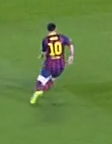
\includegraphics[width=.4\linewidth]{./images/ScreenShot2014-06-11at8-15-38PM.png}
        \captionof{figure}{En la imagen se observa la falta de resolución. Los
        bordes y los colores se tornan difusos.}
        \label{fig:barsa3}
    \end{minipage}%
    \begin{minipage}{.5\textwidth}
        \centering
        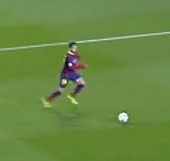
\includegraphics[width=.4\linewidth]{./images/ScreenShot2014-06-11at8-15-52PM.png}
        \captionof{figure}{La imagen muestra varias de las dificultades del
          problema. La falta de resolución, la rapidez de los movimientos y el
          diminuto tamaño de uno de los objetos de intetés: la pelota.  }
        \label{fig:barsa4}
    \end{minipage}
\end{figure}

\subsubsection{Complejidad del Análisis en Tiempo Real}

Al tener una resolución de \textit{1080p} (aproximadamente dos millones de
pixels por cuadro), el procesamiento de cada pixel debe tomar a lo sumo 20
nanosegundos.  Para lidiar con esta restricción se puede utilizar información
adicional de la que se disponga respecto al video con el objeto de evitar
procesar pixels de poca o nula utilidad para el seguimiento. Un ejemplo de esto
es descartar pixels que estén fuera de la cancha, ya que es probable que la
cámara encuadre más que el campo de juego, abarcando las gradas, el público
espectador, publicidades alrededor del campo de juego, entre otros.

Muchos autores han desarrollado algoritmos automáticos de seguimiento de
objetos en secuencias de imágenes\cite{IFTrace, alp, local-learning, MHT-2}.
Todos ellos están basados en soluciones de ecuaciones diferenciales en
derivadas parciales y resultan aceptablemente robustos, pero tienen severas
restricciones que impiden que se utilicen para aplicaciones en tiempo real.

Nuestra investigación utiliza el algoritmo de contornos
activos\cite{fast-level-set}, el cual no utiliza ecuaciones diferenciales
(haciéndolo apto para aplicaciones en tiempo real) y además hace un análisis
local () de los objetos seguidos en la imagen, lo cual hace que el tiempo de
análisis de un cuadro sea dependiente de la resolución de los jugadores e
independiente de la resolución del video.

\subsubsection{Distorsión de la lente}

Al utilizar una única cámara para captar la cancha entera se corre el riesgo de
tener distorción en los puntos de la imagen más alejados al foco de la cámara.
Este es el llamado ``efecto de ojo de buey'' e introduce mucho error, por ejemplo
en la aplicación de la homografía, por lo
tanto se debe aplicar una corrección. Una lente apropiada y bien calibrada
puede reducir este error, pero nunca puede ser eliminado totalmente. Sólo
puede evitarse utilizando una mejor técnica de filmación.

\subsubsection{Oclusiones entre jugadores}

En un partido es muy común que ocurran oclusiones entre los jugadores. El
sistema debe poder tolerar la oclusión parcial o total de los jugadores.
Esto puede llevar a situaciones muy difíciles de automatizar. Una situación
difícilmente automatizable sucede cuando dos jugadores del mismo equipo (con
vestimenta muy similar) se encuentren alineados con respecto a la cámara.
Se pueden agregar reglas para intentar que el método no se confunda, cuando
los jugadores se separen, quién es quién, pero no hay una solución evidente.

Por ejemplo, se puede utilizar información de cuadros anteriores para
estimar la velocidad de cada uno y estimar sus nuevas posiciones, pero esto
es poco efectivo si los jugadores cambian de velocidad mientras uno ocluye
al otro, o si la velocidad era muy similar al momento de generarse la oclusión.

Otra situación problemática similar es una jugada de córner, donde las
oclusiones entre varios jugadores son muy numerosas, lo que agrega a la
restricción de tiempo real mayor complejidad, ya que la resolución de
oclusiones debe ser muy eficiente en tiempo.

\subsubsection{Algoritmo utilizado}

El correcto funcionamiento del algoritmo de contornos
activos\cite{fast-level-set} depende de una buena selección de la función
característica, para poder distinguir claramente a un jugador respecto a otros
objetos o respecto del fondo. En casos como el ilustrado por la figura
\ref{fig:camiseta}, elegir una función característica resulta sencillo, ya que
con elegir el color de la camiseta se asegura una buena descripción del contorno
a seguir. Sin embargo, la imagen de la figura \ref{fig:camiseta-rayada} introduce
uno de los problemas en la selección de la función característica. Se puede ver que
las diferencias entre ambos colores del objeto hacen dificil identificarlos a ambos
con una misma caracteristica.

%TODO meter alguna referencia?
%TODO que onda las otras imagenes?
\begin{figure}[H]
    \centering
    \begin{minipage}{.5\textwidth}
        \centering
        
\includegraphics[width=.4\linewidth]{./images/rect2995.png}
        \captionof{figure}{Camiseta de color lisa. El color de la camiseta es claramente distinguible del fondo.}
        \label{fig:camiseta}
    \end{minipage}%
    \begin{minipage}{.5\textwidth}
        \centering
        
\includegraphics[width=.4\linewidth]{./images/rect2996.png}
        \captionof{figure}{Camiseta de 2 colores rayada. Las franjas de la camiseta con claramente distinguibles entre sí y el fondo.}
        \label{fig:camiseta-rayada}
    \end{minipage}
\end{figure}

Este es un desafío grande debido principalmente a dos problemas:
\begin{itemize}

\item Selección de colores: si la cancha tiene un color muy similar a la
  camiseta de un equipo, ¿cómo será posible distinguirlos? Se exploran
  distintas alternativas, como utilizar otra codificación de color.

\item Textura de los jugadores: esto representa un gran problema por varias
  razones. La primera es que la técnica de contornos activos está atada a la
  selección de una o varias características del objeto a seguir. Como la
  característica más distintiva es el color, la técnica se basá en ella. Pero
  para camisetas con más de un color, se vuelve absurda la idea de encontrar
  un color característico, dado que no existe.  Esta dificultad se ilustra en
  la imágenes de las figuras \ref{fig:barsa1} y \ref{fig:barsa2}. Por
  otro lado, dada la escasa cantidad de pixels que representan a un jugador,
  debido a nuestro enfoque de única cámara, cualquier tipo de análisis se torna
  complejo cuando sus características no están lo suficientemente definidas
  como para diferenciarlas (ya sea de otros jugadores o del fondo).

\end{itemize}

\begin{figure}[H]
    \centering
    \begin{minipage}{.5\textwidth}
        \centering
        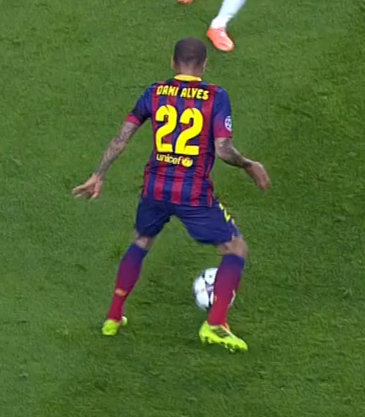
\includegraphics[width=.4\linewidth]{./images/ScreenShot2014-06-11at8-13-15PM.png}
        \captionof{figure}{Desde este punto de vista, se puede observar al menos 3 fuertes
        características (colores) en la camiseta del jugador, rojo, azul y amarillo.}
        \label{fig:barsa1}
    \end{minipage}%
    \begin{minipage}{.5\textwidth}
        \centering
        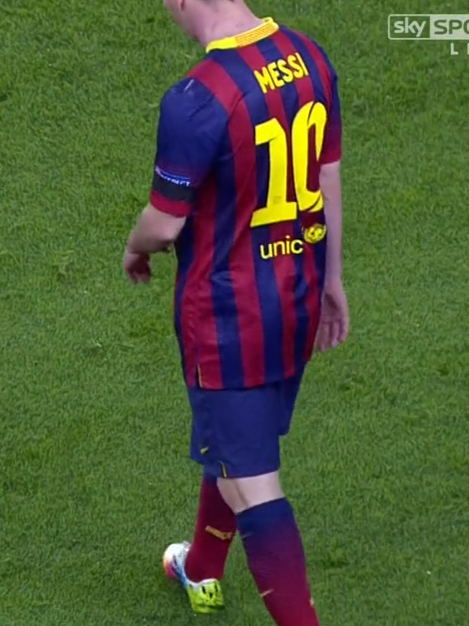
\includegraphics[width=.4\linewidth]{./images/ScreenShot2014-06-11at8-20-09PM.png}
        \captionof{figure}{Incluso con mayor resolución, las distintas características (como ser los colores azul, amarillo, y rojo) dificultan el seguimiento con contornos activos.}
        \label{fig:barsa2}
    \end{minipage}
\end{figure}

%TODO aca mepa que pueden ir varias imagenes.
% 1 de un tracking de de un jugador de remera blanca (podría ser PRE y POST, osea sin pintar y pintado)
% 1 de un tracking de un jugador de boca (again PRE y POST)
% 1 de la pelota? Para mostrar la cantidad infima de pixels?
